\documentclass[10pt, a4paper]{article}

\usepackage{graphicx}
\usepackage{float}

\begin{document}

\section{CAN questions}
\begin{enumerate}
    \item \textbf{Describe a CAN message} \newline
        A CAN message has several fields. First a 11 or 29 bit
        \textit{identifier field}. Arbitration and and prioritization is done
        here. Then comes the \textit{Control Field}, containing the
        \textit{Data Length Code}. This determines how long the message is going
        to be, 0-8. The \textit{Data Field} comes after that, followed by the
        \textit{CRC} field containing a checksum for the message. Lastly, the
        \textit{Acknowledgement Field} is set to 1 by the transmitter and is set
        to 0 by any reciever.
        \begin{figure}[H]
            \center
            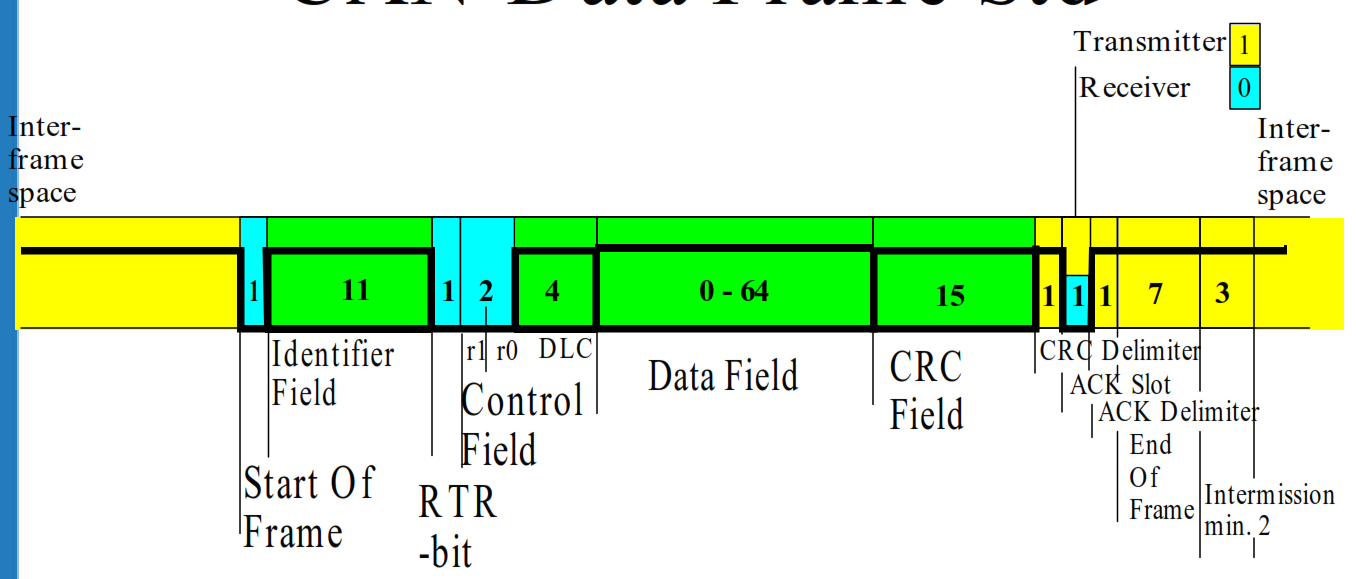
\includegraphics[scale=0.3]{canmessage.png}
            \label{fig:canmessage}
        \end{figure}
    \item \textbf{What is NRZ? How does it work?}\newline
        \textit{Non Return to Zero} means that the signal does not return to a
        zero between every bit. This means less switching than for example
        Manchester coding but it is not self clocking. 
    \item \textbf{What is bit stuffing? Worst case?}\newline
        To make sure the signal is synchronized with the clock, after five
        consecutive bits in a signal, a bit of opposite polarity is sent. This
        carries no information and is "destuffed" at the reciever. In the worst
        case scenario, there are five of the same bits sent followed by
        alternating between four of every bit after that. Bit stuffing then
        forces all bit clusters to be five of length. This would cause a 29 bit
        message to be 36 bits long, givin NRZ with bit stuffing a maximum
        overhead of $24\%$.
        \begin{figure}[H]
            \centering
            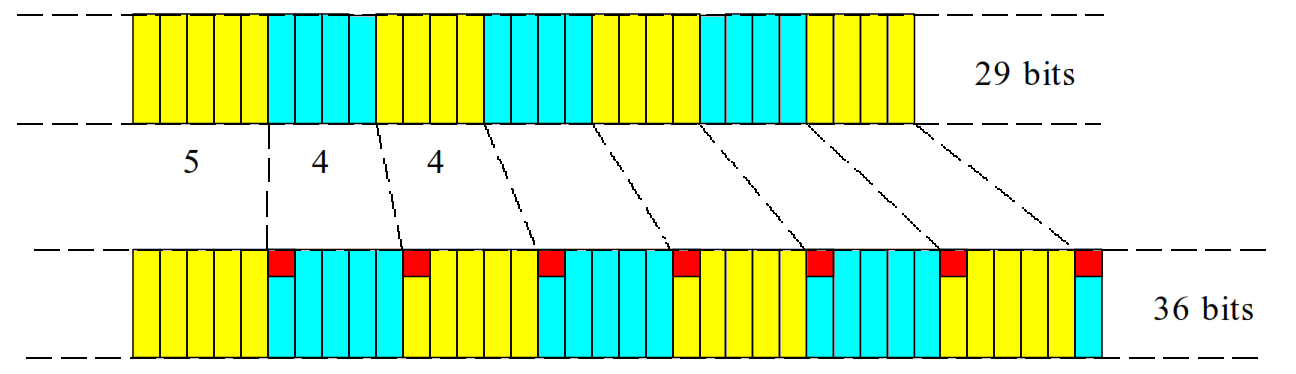
\includegraphics[scale=0.3]{bitstuff.png}
            \caption{Maximum overhead in bit stuffing}
            \label{fig:bitstuff}
        \end{figure}
    \item \textbf{How does bit timing work?}\newline
        Each bit is divided into four parts. These are \textit{Sync}, 
        \textit{Propagation}, \textit{Phase 1} and \textit{Phase 2}. Each part
        is then built up by time quantas, for a total of 4-25 time quanta per
        bit. At the sync segment, an edge is expected and the nodes on the bus
        are then synced after this. During the propagation phase, the physical
        signal is allowed to settle. The signal is sampled after phase 1. Phase
        2 is used to resynchronize the signal is a synchronization error is
        detected during the sync segment. 
    \item \textbf{What is CRC? What is a parity bit?}\newline
        CRC, or \textit{Cyclic Redundancy Checksum}, it checks so that the
        message recieved was not corrupted. The parity bit is an error check
        that counts the number of 1 bits, and returns a 1 or 0 if the number is
        odd or even.
    \item \textbf{Why do we need termination resistors? How does cable length
        affect the maximum bus speed?}\newline
        Termination resistors are used in part to prevent high frequency signal
        reglection but also to connect to $Can_+$ rail to the $CAN_-$ rail.
    \item \textbf{If two messages are being sent on the same time on the bus,
            for example 0101010101 and id 1010101010, which one is recieved and
        why?}\newline
        The first is recieved because of 0 being the dominant bit.
    \item \textbf{Describe the different Frames}\newline
        There are four types of frames in CAN. The \textit{Data Frame} is a
        frame that contains data. On the other hand, there is also the
        \textit{Remote Frame} that requests data from a specific identity. There
        are also the \textit{Error Frame} and the \textit{Overload Frame}
    \end{enumerate}
\end{document}
